\documentclass[12pt,twoside]{report}
\usepackage[utf8]{inputenc}
\usepackage{graphicx}
\usepackage{amsmath}
\usepackage{amsfonts}
%\usepackage[spanish]{babel}  %Cosas en español

% ---------------- Puntos decimales en lugar de comas para los numeros ---------------------------------
%\decimalpoint

%--------------------------------------------- Estilo de las paginas -----------------------------------
\usepackage[letterpaper,width=150mm,top=25mm,bottom=25mm,bindingoffset=6mm]{geometry}
\usepackage{fancyhdr}
\pagestyle{fancy}
\usepackage{multirow}
\usepackage{color}
\usepackage{colortbl}
\usepackage{xcolor}
\usepackage{float}
\definecolor{MSUgreen}{RGB}{0,150,150}
\fancyhead{}
\fancyhead[RE,LO]{\rightmark}
%\fancyhead[LE,RO]{\thepage}

\fancyfoot{}
\fancyfoot[CE,CO]{\thepage}


\renewcommand{\headrulewidth}{0.4pt}

%\usepackage{biblatex}
%\addbibresource{chapters/bibliografía.bib}

%--------------------------Para las citas (al menos m comprime cuando son muchas y no las pone entre comas)
\usepackage{cite}
\usepackage{varioref}
\usepackage[breaklinks,colorlinks=true, pdfstartview=FitV, linkcolor=blue, citecolor=red, urlcolor=blue]{hyperref}
%\usepackage{kantlipsum}
\usepackage{textcomp}
\usepackage{subfigure}
\usepackage{appendix}
%\usepackage{cite}           % para contraer referencias
\usepackage{longtable}      % Utilizado para la lista de simbolos
\usepackage{fancyhdr}
\usepackage{color}
\usepackage{xcolor}
\usepackage{pstricks}
%----------------------------------- Para hacer indice en panel lateral ----------------------------------
\usepackage{hyperref}
%\hypersetup{pdftex,colorlinks=true,allcolors=blue}
\usepackage{hypcap}

%-------------------------- Paquete para modificar los titulos de los cap y secciones---------------------
\usepackage{titlesec}		

%------------------------------- Lineas alrededor de los capitulos numerados -----------------------------
\titleformat{\chapter}[display]
{\Large\bfseries}
{\titlerule[4pt] \chaptertitlename\ \thechapter}{5pt}
{\large}[{\titlerule[2pt]}]


%------------------------------- Lineas alrededor de los capitulos no numerados -----------------------------
\titleformat{name=\chapter,numberless}[display]
{\Large\bfseries}
{\titlerule[4pt]}{-20pt}
{\large}[{\titlerule[2pt]}]

\titlespacing*{\chapter}{0pt}{30pt}{20pt}

%\usepackage[nottoc,numbib]{tocbibind}


\graphicspath{ {./Figures/} }
\lhead{Modeling properties of the double exchange model hamiltonian}
\rhead{M2 Internship}
%\lfoot{TODO 1}
%\rfoot{TODO 1}
%\def\changemargin#1#2{\list{}{\rightmargin#2\leftmargin#1}\item[]}
%\let\endchangemargin=\endlist
\title{Modeling properties of the double exchange model hamiltonian}

\newcommand{\citepetsc}{\cite{petsc_web_page,petsc_user_ref,petsc_efficient}}
\newcommand{\citeslepc}{\cite{Hernandez_2003_SSL,slepc_users_manual}}





\begin{document}
	\begin{titlepage}
		\begin{center}
			%\vspace{-2cm}
			
\includegraphics[width = 0.2\textwidth]{lcpq.png} \hspace{0.5cm}
			
\includegraphics[width = 0.2\textwidth]{irsamac.png} \hspace{0.5cm}
			
\includegraphics[width = 0.2\textwidth]{ups.png} \hspace{0.5cm}
			
\includegraphics[width = 0.25\textwidth]{TCCM.png} \\
			\vspace{1cm}
			\Large
			{Master studies in Theoretical Chemistry and Computational Modelling\\
				Laboratoire de chimie et physique quantiques\\
				Université Toulouse III - Paul Sabatier\\
				%\end{center}
				
				%\includegraphics[width = 0.10\textwidth]{insteclogo} \hspace{2cm}
				
				%\includegraphics[width = 0.10\textwidth]{UH_logo.png} \\
				\vspace{-0.5cm}
				
				
				
				%\vspace{0.5cm}		
				
				
				
				\vspace{2cm}
				\Huge
				\textbf{ \color{MSUgreen} Modeling properties of the double exchange model hamiltonian }
				
				\vspace{3cm}
				\Large
				\begin{tabular}{l l}			
					{\bf Author:}   & Jos\'e David Crem\'e \\[1cm]
					{\bf Supervisors:} & Vijay G. Chilkuri \\
					& Nicolas Suaud
				\end{tabular}
			}
			
			\vspace{3cm}
			\Large
			Toulouse, 2023 \\
			
			\vspace{0.8cm}
			
		\end{center}
	\end{titlepage}
	%\maketitle
	%\thispagestyle{empty}
	\setcounter{page}{1}
	\tableofcontents
	\chapter*{Introduction}
	\addcontentsline{toc}{chapter}{Introduction}
	
	Introduce the following topics
	\begin{itemize}
		\item Colossal magnetic resistance
		\item Anomalous behavior of magnetic susceptibility in linear chain of Nickelates
	\end{itemize}
	
	\section*{Experimental studies}
	\addcontentsline{toc}{section}{Experimental studies}
	
	One dimensional transition metal chains have been synthesized and studied in
	literature.~\cite{darriet_compound_1993,batlogg_haldane_1994} Experimental
	studies on 1D Nickelates have shown that they exhibit a magnetic field
	dependence in their resistivity upon doping.\cite{xu_holes_2000} Here, we focus
	on the low temperature behavior of the 1D doped Nickelates close to the curie
	temperature. Experimental studies of susceptibility of 1D doped Nickelates have
	shown that near the Curie temperature, the materials show antiferromagnetic
	behavior.\cite{Ramirez} This behavior is contrary to the usual double exchange
	model where the holes are mobile throughout the chain. We develop arguments and
	discuss some new ideas to explain this behavior of the magnetic susceptibility
	in 1D doped Nickelates.
	
	\section*{Theoretical studies}
	\addcontentsline{toc}{section}{Theoretical studies}
	
	One dimensional transition metal chains are immencely useful models
	for theoretical analysis due to the existance of powerful techniques
	such as the density matrix renormalization group (DMRG) and lanczos
	exact diagonalization techniques. Such methods can be applied to
	high accuracy and have been used to study models similar to the
	one studied here but with important differences.\cite{dagotto_correlated_1994,patel_emergence_2020}
	Further work by Dagotto. et. al have shown details of the existance
	of a ferromagnetic polaron and its extent in such 1D models.\cite{malvezzi_origin_2001} However, the parameter range
	that we have chosen for the current study relies on those extracted
	by \textit{ab initio} calculstions on Nickel dimers.\cite{bastardis_microscopic_2007,bastardis_isotropic_2008}
	Therefore, the present study serves to augment the available literature
	for parameter range extracted using \textit{ab initio} calculations.
	
	\chapter{Double Exchange Hamiltonian}
	
	The double exchange model is used to describe mixed lvalent transition
	metal based molecules. The phenomenology of ferromagnetic and anti-ferromagnetic
	behavior in such molecules is captured by the various parameters of the
	double exchange model Hamiltonian (Eq:~\ref{eq:demodel}).
	
	\begin{equation}
		\begin{split}
			\hat{H} & = \sum_i 2K \hat{S}_{a_i}\cdot\hat{S}_{b_i} 
			+ \sum_{ij} 2J_a \hat{S}_{a_i}\cdot\hat{S}_{a_j} 
			+ \sum_{ij} t\left( \hat{c}^{\dagger}_{a_i}\cdot\hat{c}_{a_j} + \text{h.c.}\right ) \\
		&	+ \sum_{i,i+1} V_{NN}\left ( \delta_{n_i,0}\ \delta_{n_{i+1},0} \right ) 
			+ \sum_{i,i+2} V_{NNN}\left ( \delta_{n_i,0}\ \delta_{n_{i+2},0} \right )
		\end{split}
		\label{eq:demodel}
	\end{equation}
	
	The above Hamiltonian describes a model with two valence orbitals on each
	atom (site) ideally of differnet symmetry (i.e. orthogonal, e.g. $a,b$). A schematic is shown in
	Figure:~\ref{fig:deham}.
	
	%\begin{figure}[ht]
	%	\centering
	%	\begin{modiagram}[names]
	%		\atom[$1$]{left}{
	%			1s = { 0; up} ,
	%			2s = { 1; up} ,
	%		}
	%		
	%		\atom[$2$]{right}{
	%			1s = { 0; up} ,
	%			2s = { 1;   } ,
	%		}
	%		\node[right,xshift=4mm] at (1sright) {$b$};
	%		\node[right,xshift=4mm] at (2sright) {$a$};
	%		\node[left,xshift=-4mm] at (1sleft) {$b$};
	%		\node[left,xshift=-4mm] at (2sleft) {$a$};
	%		
	%		\draw[<-,gray,semithick]   (2sright) edge[bend right] node [left] {} (2sleft);
	%		\draw[<->,gray,semithick] (1sright) edge[bend left] node [left] {} (1sleft);
	%		\draw[<->,gray,semithick] (1sleft) edge[bend left] node [left] {} (2sleft);
			
	%		\node[left,xshift=2.3cm, yshift=-9mm] at (1sleft) {$J$};
	%		\node[left,xshift= 4mm, yshift=5mm] at (1sleft) {$K$};
	%		\node[left,xshift=2.3cm, yshift=-0mm] at (2sleft) {$t$};
			
	%	\end{modiagram}
	%	\caption{\label{fig:deham} Orbital diagram representing the mail interactions of the double exchange model with two valence orbitals on each atom.}
	%\end{figure}&
	
	In Eq:~\ref{eq:demodel}, the spins of the electrons are represented by $S_a$,
	where the subscript $a$ denotes the orbital on which the electron resides.  The
	creation and annahilation operators of electrons are represented by
	$\hat{c}^{\dagger}$ and $\hat{C}$ respectively. The parameters in the model
	Hamiltonian are defined as follows:
	
	\begin{itemize}
		
		\item $K$ - The local exchange integral. This exchange integral represents
		Hund's rule and is always positive. The local exchange favors parallel
		coupling i.e. a local high spin determinant.
		
		\item $J$ - The kinetic exchange interaction between orbitals of symmetry $a$
		on neighboring sites. This integral is responsible of the anti-parallel coupling.
		
		\item $t$ - The kinetic energy integral or the hopping term. The
		transfer of electrons from one atom to the neighboring atom is represented
		by the hopping term. This also favors parallel coupling when taken along with
		the exchange integral $K$.
		
		\item $V$ - The hole repulsion term. This takes into account the repulsion between
		holes which are on neighboring sites $V_{NN}$ or next-nearest neighboring sites $V_{NNN}$. The hole repulsion indirectly takes into account the repulsion between
		electrons occupying nearby sites.\cite{calzado_proposal_2001}
		
	\end{itemize}
	
	\section{Parameter Space}
	
	All the parameters of the model are important for understanding the collective
	properties of the double exchange hamiltonian. Here we give the order of magnitude
	of all the parameters used keeping in mind that we target molecules based on
	transition metal atoms.
	Previous studies using \textit{ab initio} methods in order to extract model
	parameters for various transition metal atoms such as Cu, Mn, and Ni have
	provided realistic order of magnitudes of the values of the parameters.
	In the present analysis, we use the full range of values in order to represent
	the full range of transition metal atoms.
	
	\begin{table}[h!]
		\centering
		\begin{tabular}{||c||}
			\hline
			Parameters  \\ [0.5ex]
			\hline\hline
			\\
			$ 0.01\lvert t \rvert \le J \le 0.15\lvert t \rvert $    \\ [1ex]
			$ 0.01\lvert t \rvert \le J \le 0.15\lvert t \rvert $    \\ [1ex]
			$ 0.4 \le K \le 0.8 $                                    \\ [1ex]
			$ V_{NN} = \frac{\alpha}{2r}\ ;\ 0.5 \le \alpha \le 0.8 $ \\ [1ex]
			$ V_{NNN} = \alpha V_{NN} $                                \\ [1ex]
			\hline
		\end{tabular}
		\label{tab:params}
		\caption{Table with range of parameter values.}
	\end{table}
	
	Including the hole repulsion term significantly changes the low energy physics
	of the model as shown by previous work\cite{calzado_proposal_2001}. Here we will
	study the influence in the variation of all the above parameters.
	
	
	\chapter{Methodology}
	
	The double exchange hamiltonian is studied for one dimensional chain
	of sites containing holes with a doping ratio of 1:3 i.e. one hole for every
	three sites. This follows our previous study which shows that for
	the physically meaningful range of parameter values (Table:~\ref{tab:params}),
	a single hole aligns about three sites.\cite{crystals_chilkuri}
	
	\section{Exact diagonalization}
	
	An exact diagonalization method is used to obtain many low energy states of the
	hamiltonian. Due to the exponential growth of the hilbert space with the number
	of sites, exact diagonalization becomes challenging.Here we use our home made
	code relying on PETSc\citepetsc and SLEPc\citeslepc libraries to perform exact diagonalization and
	use a large number of high performance compute nodes for distributed storage of
	the hamiltonian matrix and eigenvectors. We have used DEHam\cite{deham} to
	perform exact diagonalization of very large number of sites up to 18 sites
	containing 36 orbitals with 6 holes which corresponds to a hilbert space of
	about $0.5 \times 10^9$ determinants.
	
	\section{Model space}
	
	\section{Model Hamiltonian}
	
	\section{Projector}

	\subsection{Spatial part}

	The spatial part of the projector is taken from the diagonalization of a
	Hueckel hamiltonian for three sites which is given below:

	\begin{equation}
		\begin{split}
			 \begin{pmatrix}
			   0 & t & 0 \\
			   t & 0 & t \\
			   0 & t & 0 \\
			 \end{pmatrix}
		\end{split}
		\label{eq:demodel}
	\end{equation}

	The basis are the three determinants possible for on hole and two particles,
	i.e. $|bc\rangle,|ac\rangle,|ab\rangle$.  Diagonalization of this
	hamiltonian gives the lowest energy eigenvector given below, which is used
	as the projector for the spatial part of the wavefunction inside each region
	composed of one hole and three sites.

	\begin{equation}
		\begin{split}
		  |\phi_{i}\rangle = \frac{1}{2}\left| bc\right\rangle +
\frac{\sqrt{2}}{2}\left| ac\right\rangle +
\frac{1}{2}\left| ab\right\rangle
		\end{split}
		\label{eq:demodel}
	\end{equation}

	The full projector is simply the tensor product of the above projector
	on all the box regions given as follows.

	\begin{equation}
		\begin{split}
			\hat{\mathcal{P}}_{space} & = \bigotimes_{i = 1}^{m}\left|\phi_i\right\rangle
		\end{split}
		\label{eq:demodel}
	\end{equation}

	\subsection{Spin part}

	The spin part of the projector for two sites is defined as follows:


	\begin{equation}
		\begin{split}
			\hat{\mathcal{P}}_{spin}(S_T,M_{S_T}) & = \sum_{M_{S_R}}\sum_{M_{S_L}} \begin{pmatrix} \frac{5}{2} & \frac{5}{2} & S_T\\ M_{S_R} & M_{S_L} & M_{S_T} \end{pmatrix}\left |\frac{5}{2},M_{S_R}\right\rangle\otimes\left|\frac{5}{2},M_{S_L}\right\rangle
		\end{split}
		\label{eq:demodel}
	\end{equation}

	where $S_T$ and $M_{S_T}$ represent the total spin and the total $Ms$
	respectively. The values $M_{S_L}$ and $M_{S_R}$ represent the $Ms$ of the
	$\frac{5}{2}$ spins on the left and right respectively. The values in
	brackets represent Clebsch Gordan coefficients (CGC) for the three spins
	entering the couping formula.  The wavefunction is a tensor product of all
	the possible $Ms$ combinations generated by two $\frac{5}{2}$ spins.

	Similarly, the projector for an arbitrary number of sites si similarly defined
	as follows:

	\begin{equation}
		\begin{split}
			\hat{\mathcal{P}}_{spin}(S_T,M_{S_T}) & = \sum_{M_{S_i}}\dots\sum_{M_{S_m}} \prod_{i}^{m} \begin{pmatrix} \frac{5}{2} & \frac{5}{2} & S_T\\ M_{S_i} & M_{S_{i+1}} & M_{S_T} \end{pmatrix}
			\bigotimes_{i = 1}^{m}\left|\frac{5}{2},M_{S_i}\right\rangle
		\end{split}
		\label{eq:demodel}
	\end{equation}

	In this way, the spin part of the projector on the model space can be uniquely
	defined for an arbitrary number of sites.

	The total projector can then be written as the product of the spin
	and spatial parts given above.

	\begin{equation}
		\begin{split}
			\hat{\mathcal{P}} & = \hat{\mathcal{P}}_{space}\otimes\hat{\mathcal{P}}_{spin}
		\end{split}
		\label{eq:demodel}
	\end{equation}
	
	\section{Effective Hamiltonian}
	
	%\section{Real Space Renormalization Group}
	
	\begin{chapter}{Results and discussion}
	
	%\section{Hole repulsion}
	
	%TODO
	
	\section{Weight vs $J$}
	\subsection{Variation with the number of sites}
	\begin{figure}[ht]
		\centering
		\hspace{-1.5cm}
		\begin{minipage}{0.4\textwidth}
			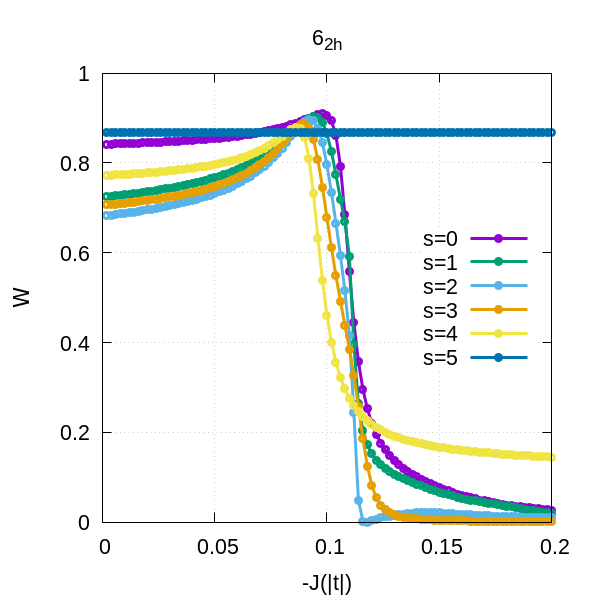
\includegraphics[scale=0.4]{W_vs_J_sites_2-xrep-0.png}
		\end{minipage}
		\hspace{2cm}
		\begin{minipage}{0.4\textwidth}
			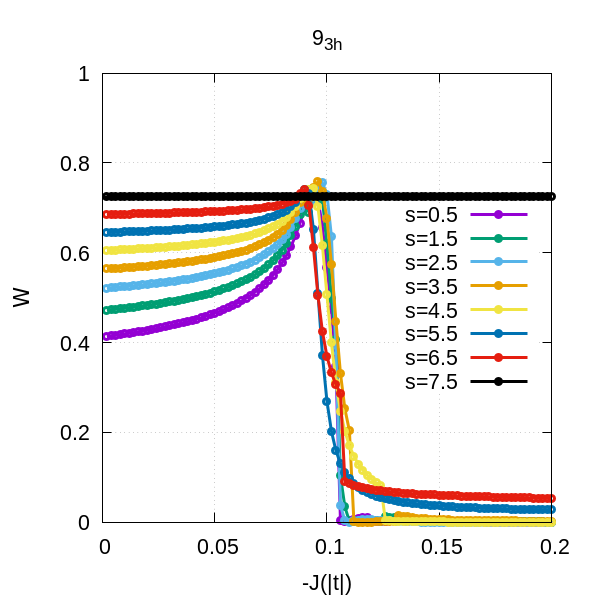
\includegraphics[scale=0.4]{W_vs_J_sites_3-xrep-0.png}
		\end{minipage}
		\caption{\label{fig_w69} Weight (W) as a function of $J$ for 6$_{2h}$ (left) and 9$_{3h}$ (right). }
	\end{figure}
	Figure \ref{fig_w69} shows the weight of the wave function projected in the model space as afunction of J for 6$_{2h}$ (left) and 9$_{3h}$ (right), for each value of spin is represented the one with a bigger weight. This confirms that it is possible to have an interval of values of J in which the weight reach excellent values (even $>$ 90$\%$ in some cases). It is possible to see that weights for 9$_{3h}$ are smaller than those of 6$_{2h}$ this due to the fact that when increasing the size of the system it also increase the number of determinants out of the model space. However this decreasing in the weight is is expected to converge in the thermodinamyc limit, in fact, the sum of the weights over all the determinants is 1 as it is an orthonormal space. In all the cases the highest spin state does not depend on $J$.
	 
	 In a first moment weight increases with $J$ this is because for a small value of $J$ the system is completely governed by $t$ and that will favor the ionic determinants, but after the weight falls drastically as J favors the antiferromagnetic couplings inside the boxes.
	
	
	\subsection{Variation with Repulsion}
	\begin{figure}[h!]
		\centering
		\hspace{-2cm}
		\begin{minipage}{0.4\textwidth}
			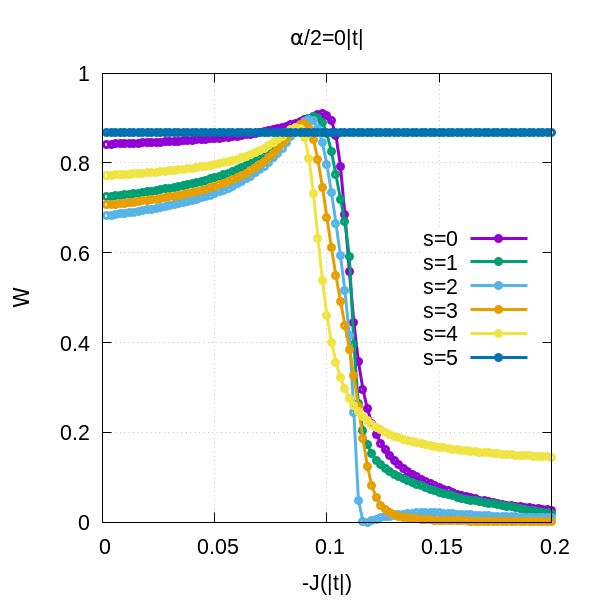
\includegraphics[scale=0.4]{W_vs_J_sites_2-xrep-01.png}
		\end{minipage}
		\hspace{2cm}
		\begin{minipage}{0.4\textwidth}
			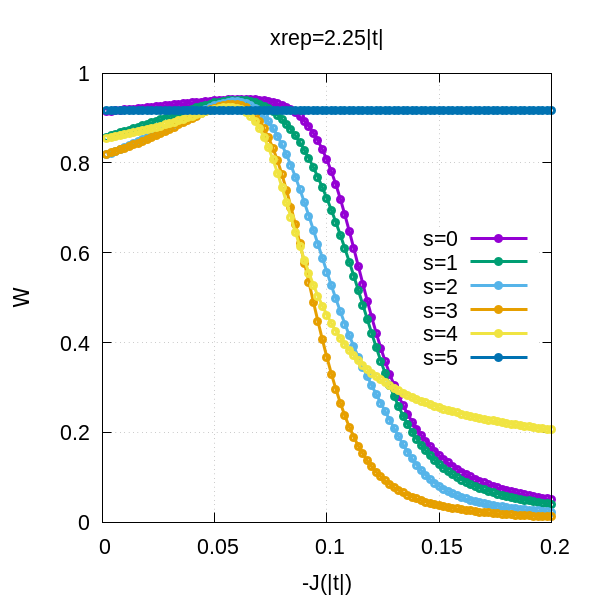
\includegraphics[scale=0.4]{W_vs_J_sites_2-xrep-225.png}
		\end{minipage}
		\caption{\label{fig_0_225} Weight (W) as a function of $J$ for xrep=0 $|t|$ (left) and xrep=2.25 $|t|$ (right). }
	\end{figure}
	
	In figure \ref{fig_0_225} are shown the weight as a function of $J$ without hole repulsion (left) and a hole repulsion with $\alpha=2.25|t|$ (right). Here it is possible to see the same tendence but repulsion increases the weight in the model space as it forces the holes away from each other and this decreases the weight of the ionic determinants. 
	
	\section{Influence of hole repulsion}
	\subsection{Variation of maximal weight}
	In order to better understand the effect of hole repulsion it is convenient to analize the maximal value of weight for each state for several values of $\alpha$ as displayed in figure \ref{fig_v1n} for two models: at left only considering repulsion between first neighbors and at right repulsion between all the holes as a function of distance. At the begining there is an increase of the weight as explained above but for bigger values of repulsion there is a slight decrease as it will force the holes to be at the borders, and the spatial projector is the solution of Hückel in wich the hole at the exterior border of each box has a weight of 25$\%$, so even if itgains in weight the decreasing of the others will cause a global but slight decrease.So with $\alpha=2.25|t|$ we have the maximal values of weight.  
	
	\begin{figure}[h!]
		\centering
		\hspace{-2cm}
		\begin{minipage}{0.4\textwidth}
			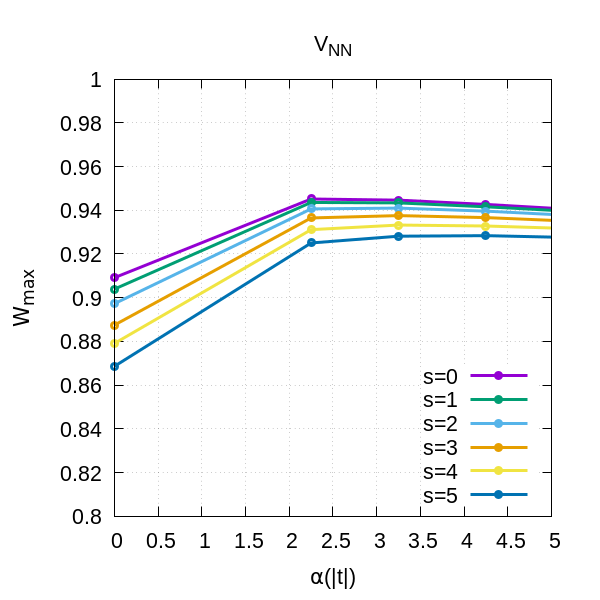
\includegraphics[scale=0.4]{Wmax_vs_xrep0v1.png}
		\end{minipage}
		\hspace{2cm}
		\begin{minipage}{0.4\textwidth}
			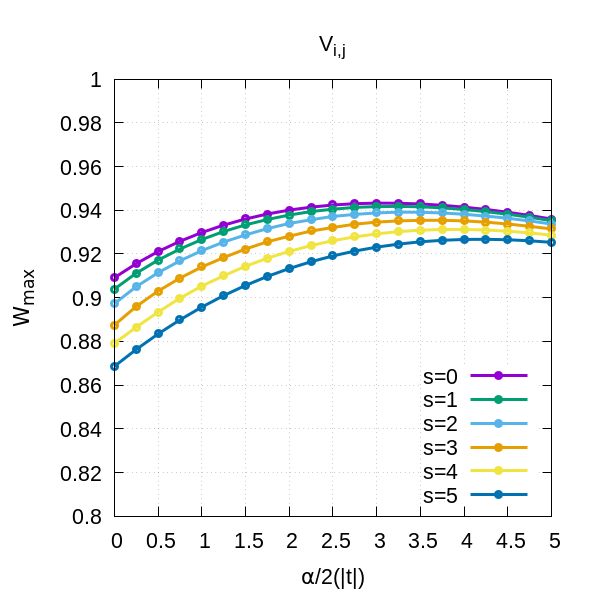
\includegraphics[scale=0.4]{Wmax_vs_xrep0vn.png}
		\end{minipage}
		\caption{\label{fig_v1n} Maximal weight (W$_{max}$)as a function of repulsion calculated with two models: only considering repulsion between consecutive holes (left) and considering repulsion between all the holes as function of distance (right). }
	\end{figure}
	
	\subsection{Impact on $J$ and $t$}
	\begin{figure}[h!]
		\centering
		\hspace{-2cm}
		\begin{minipage}{0.4\textwidth}
			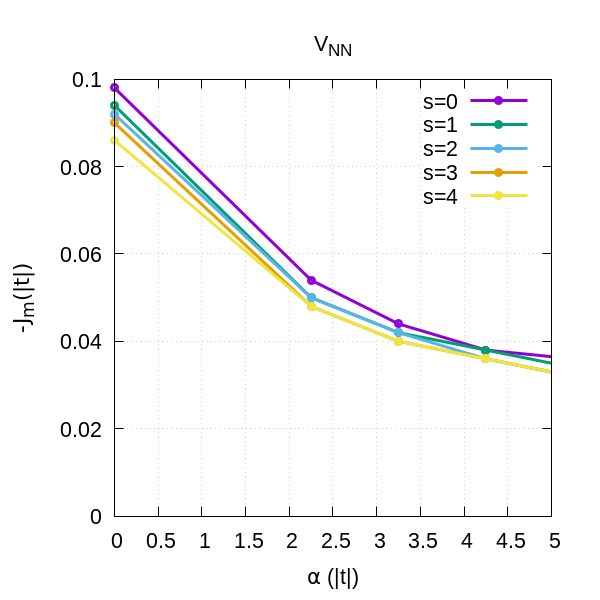
\includegraphics[scale=0.38]{J_vs_xrepv1.png}
		\end{minipage}
		\hspace{2cm}
		\begin{minipage}{0.4\textwidth}
			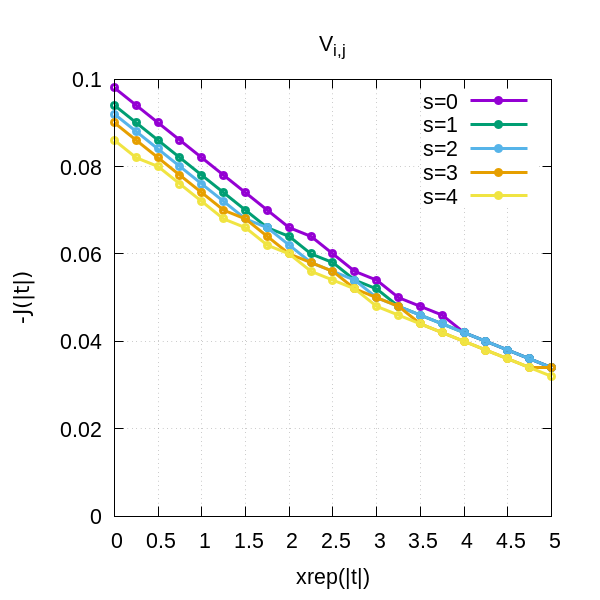
\includegraphics[scale=0.38]{J_vs_xrepvn.png}
		\end{minipage}
		\caption{\label{fig_jv1n} Value of $J$ for which the maximal weight is reached ($J_m$) as a function of repulsion calculated with two models: only considering repulsion between consecutive holes (left) and considering repulsion between all the holes as function of distance (right). }
	\end{figure}
	Repulsion decreases the kinetic energy of the system as it constrains the movement of holes, this will have a direct impact in the effect of $t$. As we pointed before there is a competition between $J$ (which favors antiferromagnetic coupling) and $t$ (which favors ferromagnetic coupling), so this negative impact of repulsion on the effect of $t$ will cause that for even smaller values of $J$ the ferromagnetic coupling becomes stronger and makes the weight falls abruptely as discussed in section 3.1.1. Therefore the maximal value of weight is reached for smaller values of $J$ as shown in figure \ref{fig_jv1n} in which it is possible to see the value of $J$ for which the maximal weight is reached for several values of $\alpha$ and also for the two models explained above.
	%\subsection{RSRG}
	
	\section{Results of $J_{eff}$}
	\subsection{Influence of the number of sites}
	\begin{figure}[h!]
		\centering
		\hspace{-2cm}
		\begin{minipage}{0.4\textwidth}
			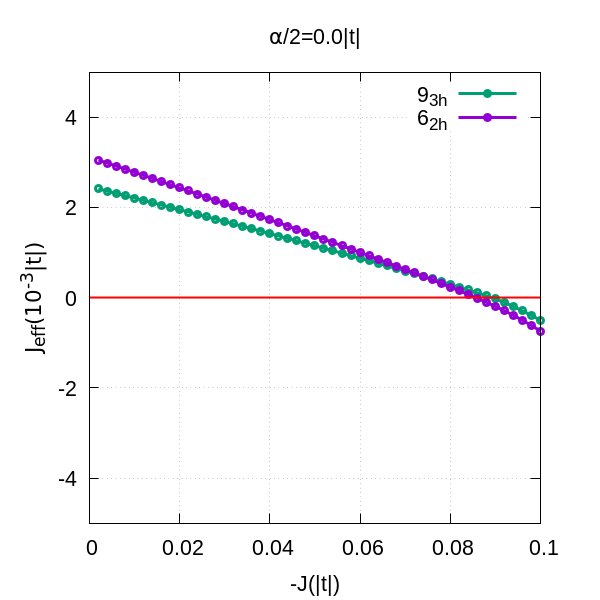
\includegraphics[scale=0.4]{Jeff_vs_J_sites_3-xrep-0.png}
		\end{minipage}
		\hspace{2cm}
		\begin{minipage}{0.4\textwidth}
			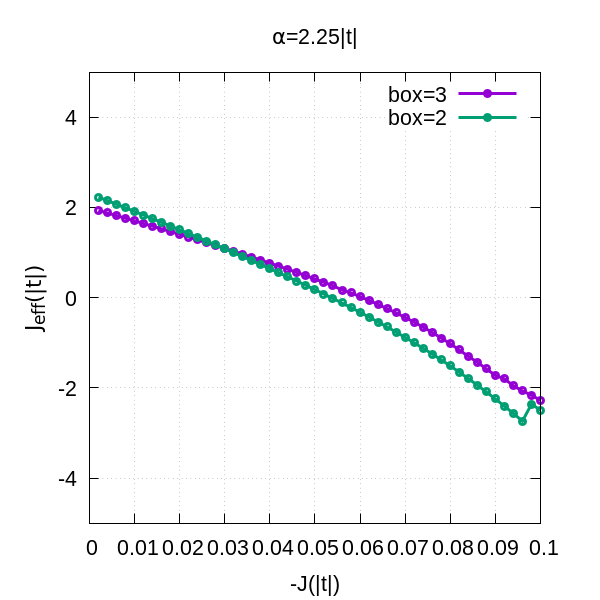
\includegraphics[scale=0.4]{Jeff_vs_J_sites_3-xrep-225.png}
		\end{minipage}
		\caption{\label{fig_arj} Value of $J_{eff}$ as a function of $J$ for $\alpha=0|t|$ (left) and $\alpha=2.25|t|$ (right). }
	\end{figure}

	
	
	
	\subsection{Influence of hole repulsion}
	\begin{figure}[h!]
		\centering
		\hspace{-2cm}
		\begin{minipage}{0.4\textwidth}
			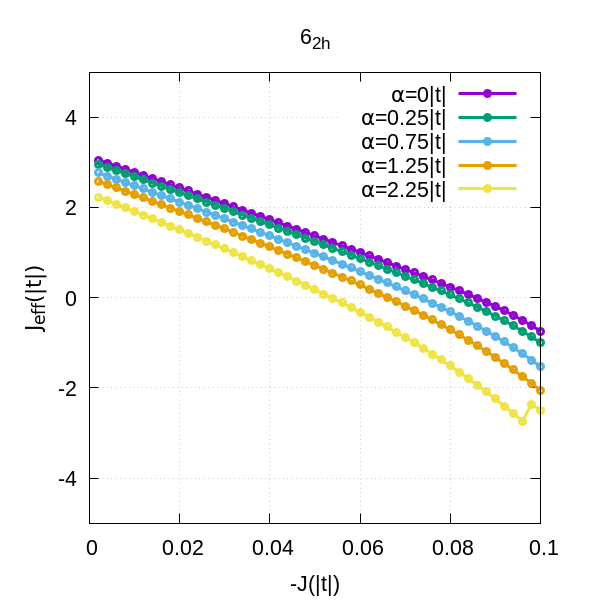
\includegraphics[scale=0.4]{Jeff_vs_J_ar2.png}
		\end{minipage}
		\hspace{2cm}
		\begin{minipage}{0.4\textwidth}
			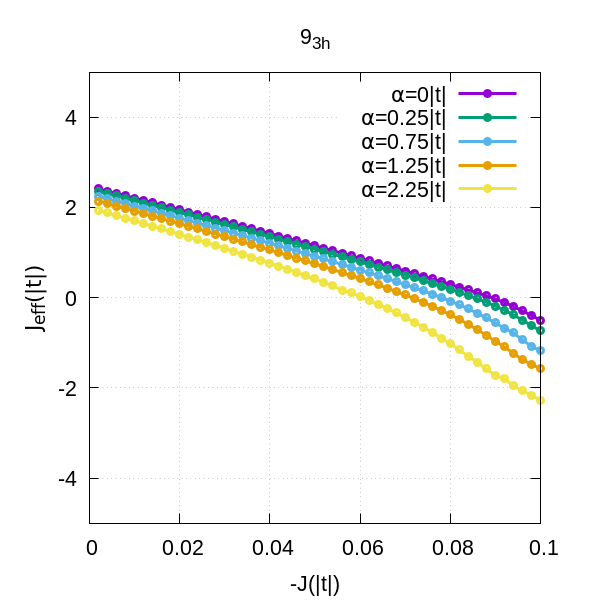
\includegraphics[scale=0.4]{Jeff_vs_J_ar3.png}
		\end{minipage}
		\caption{\label{fig_arj} Value of $J_{eff}$ as a function of $J$ for 6$_{2h}$ (left) and 6$_{2h}$ (right). }
	\end{figure}
	
	\begin{figure}[h!]
		\centering
		\hspace{-2cm}
		\begin{minipage}{0.4\textwidth}
			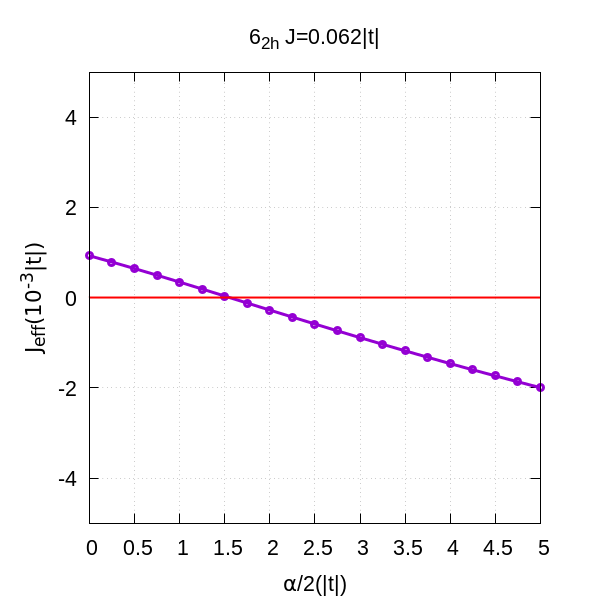
\includegraphics[scale=0.4]{Jeff_vs_xrep_ar2.png}
		\end{minipage}
		\hspace{2cm}
		\begin{minipage}{0.4\textwidth}
			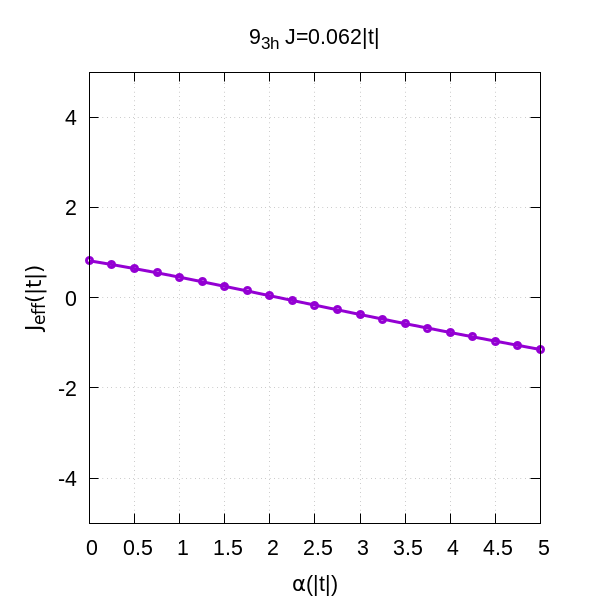
\includegraphics[scale=0.4]{Jeff_vs_xrep_ar3.png}
		\end{minipage}
		\caption{\label{fig_arxrep} Value of $J_{eff}$ as a function of $\alpha$ for 6$_{2h}$ (left) and 6$_{2h}$ (right). in both cases $J=0.062 |t|$ }
	\end{figure}
	\end{chapter} %{Discussion}
	
	\chapter*{Conclusions}
	\addcontentsline{toc}{chapter}{Conclusions}
	%\end{chapter}
	\newpage
	\pagenumbering{roman}
	\renewcommand{\bibname}{References}
	%\chapter*{References}
		\bibliography{biblio} % Use the example bibliography file sample.bib
	\bibliographystyle{unsrt} % Plain referencing style
	\addcontentsline{toc}{chapter}{References}
		\pagenumbering{roman}
		\setcounter{page}{2}

\end{document}



%*************************************************************************
% Bibliographies
%*************************************************************************
%\printbibliography
\bibliography{biblio.bib} % Use the example bibliography file sample.bib
\bibliographystyle{plain} % Plain referencing style
